\documentclass[11pt]{article}

% =====================================================================
%  Idea Validation -- Completed Frameworks
%  Project: Autonomous TEC-AWH PV-cleaning robot (graduation project)
%  Author : Rahma Elhamouly
%  Built by applying the four templates in exhibition/here.pdf
%  (Desirability/Feasibility/Viability, Empathy, Problem Statement,
%   Impact Statement) to this project.
% =====================================================================

\usepackage[a4paper,margin=1.8cm]{geometry}
\usepackage[T1]{fontenc}
\usepackage{lmodern}
\usepackage{xcolor}
\usepackage{tikz}
\usetikzlibrary{positioning,calc}
\usepackage{enumitem}
\usepackage{booktabs}
\usepackage{array}
\usepackage{parskip}
\usepackage[hidelinks]{hyperref}

% ---- palette (matched to the source slides) -------------------------
\definecolor{slideblue}{HTML}{1F4E79}   % headings
\definecolor{userblue}{HTML}{2F9BD8}    % USERS
\definecolor{needred}{HTML}{D9543B}     % NEEDS
\definecolor{insightgreen}{HTML}{7DA640}% INSIGHTS
\definecolor{feas}{HTML}{F2D55C}        % Feasible
\definecolor{desir}{HTML}{F5C518}       % Desirable
\definecolor{viab}{HTML}{F39C12}        % Viable
\definecolor{panelgrey}{HTML}{F2F4F7}
\definecolor{inkgrey}{HTML}{444444}

\setlength{\parskip}{4pt}
\renewcommand{\arraystretch}{1.3}

% ---- section heading style ------------------------------------------
\newcommand{\framehead}[2]{%
  \par\vspace{6pt}%
  {\color{slideblue}\large\bfseries #1}%
  \hfill{\color{inkgrey}\small\itshape #2}\par
  {\color{slideblue}\rule{\linewidth}{1.2pt}}\par\vspace{2pt}}

% ---- colored title panel (title bar + body) -------------------------
\newcommand{\panel}[3]{% #1 color  #2 title  #3 body
  \colorbox{#1}{\parbox[t]{\dimexpr\linewidth-2\fboxsep}{%
      \color{white}\bfseries\strut #2}}\\[-1pt]
  \fcolorbox{#1}{white}{\parbox[t]{\dimexpr\linewidth-2\fboxsep}{%
      \footnotesize\color{inkgrey}\strut #3}}}

\begin{document}
\pagestyle{empty}

% =====================================================================
%  TITLE
% =====================================================================
\begin{center}
  {\color{slideblue}\Huge\bfseries Idea Validation}\\[4pt]
  {\color{inkgrey}\large Completed innovation frameworks for the graduation project}\\[8pt]
  {\large\bfseries Autonomous Self-Watering PV-Cleaning Robot}\\[2pt]
  {\color{inkgrey} Thermoelectric atmospheric water harvesting (TEC-AWH) + autonomous panel cleaning}\\[6pt]
  {\small Rahma Elhamouly \quad$\bullet$\quad REE\,598 Graduation Project \quad$\bullet$\quad \today}
\end{center}

\noindent\colorbox{panelgrey}{\parbox{\dimexpr\linewidth-2\fboxsep}{%
\small\textbf{The idea in one line.} An autonomous rail-guided robot that cleans
photovoltaic panels \emph{while generating its own distilled cleaning water from the
surrounding air} using a thermoelectric (Peltier) atmospheric-water-harvesting module ---
engineered for Egypt's new sustainable cities at three scales: \textbf{commercial
rooftops}, \textbf{residential rooftops}, and \textbf{solar street-lighting}.}}

% =====================================================================
%  1. DESIRABILITY / FEASIBILITY / VIABILITY
% =====================================================================
\framehead{1.\ \ Desirable\,/\,Feasible\,/\,Viable}{The ``sweet spot'' --- Strategyzer, \emph{Testing Business Ideas}}

\begin{center}
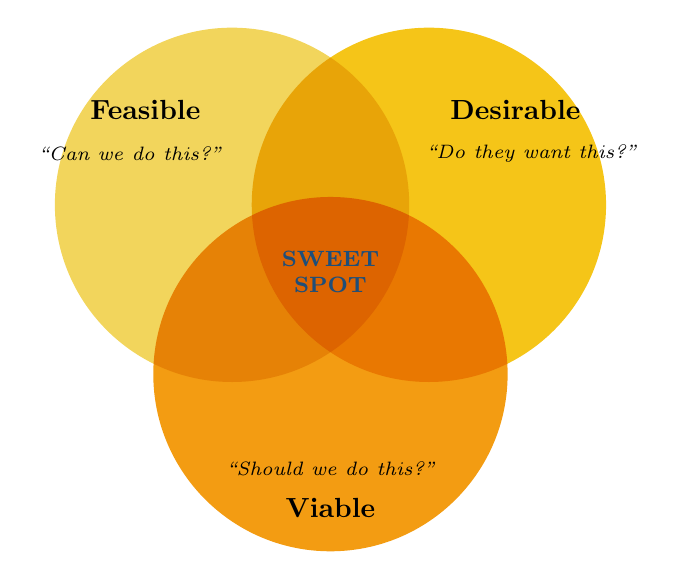
\begin{tikzpicture}[scale=1.0]
  \def\r{2.25}
  \begin{scope}[blend group=multiply]
    \fill[feas]  (-1.25, 0.9) circle (\r);
    \fill[desir] ( 1.25, 0.9) circle (\r);
    \fill[viab]  ( 0.0,-1.25) circle (\r);
  \end{scope}
  \node[font=\bfseries] at (-2.35, 2.1) {Feasible};
  \node[font=\bfseries] at ( 2.35, 2.1) {Desirable};
  \node[font=\bfseries] at ( 0.0,-2.95) {Viable};
  \node[font=\scriptsize\itshape] at (-2.55, 1.55) {``Can we do this?''};
  \node[font=\scriptsize\itshape] at ( 2.55, 1.55) {``Do they want this?''};
  \node[font=\scriptsize\itshape] at ( 0.0,-2.45) {``Should we do this?''};
  \node[align=center,font=\bfseries\footnotesize,text=slideblue]
       at (0,0.05) {SWEET\\SPOT};
\end{tikzpicture}
\end{center}

\vspace{2pt}
\noindent
\begin{minipage}[t]{0.325\textwidth}
\panel{feas}{Feasible — ``Can we do this?''}{%
Built entirely from off-the-shelf parts (TEC1-12706 tiles, V-slot gantry +
OpenBuilds plate, GA25 geared motor, ESP32, diaphragm pump); the bench prototype
parts are \textbf{already procured} ($\approx$\,4{,}150~EGP spent). TEC condensation
checked against Benban climate (RH 25--55\%, $T$ 25--42\,$^\circ$C); cleaning-water
duty sized at 1.8~L/m\textsuperscript{2}/event.\\[2pt]
\textit{Riskiest:} night-time water yield at low RH + hot-side heat rejection
$\rightarrow$ test with a 24\,h condensate run, CPU-cooler hot side, TECs PWM'd to
$\sim$70\%.}
\end{minipage}\hfill
\begin{minipage}[t]{0.325\textwidth}
\panel{desir}{Desirable — ``Do they want this?''}{%
PV operators in Egypt's desert sites lose generation to dust \emph{continuously} and
already pay for cleaning crews and trucked water. The pull: cut soiling losses
\textbf{without} spending scarce water or sending workers onto hot roofs.\\[2pt]
\textit{Evidence to gather:} O\&M interviews (NREA / Benban developers) and
rooftop-solar owners.\\[2pt]
\textit{Riskiest:} will owners trust an unattended robot on the array?
$\rightarrow$ one-rooftop pilot + 3 interviews.}
\end{minipage}\hfill
\begin{minipage}[t]{0.325\textwidth}
\panel{viab}{Viable — ``Should we do this?''}{%
Value $=$ avoided trucked-water cost $+$ avoided labour $+$ recovered generation
(soiling losses returned to the grid). Self-generated water LCOW
$\approx$\,14~USD/m\textsuperscript{3} (VCR route), to be weighed against trucked
water plus the recovered kWh. Model: cleaning-as-a-service or unit sale to plant
owners / new-city authorities.\\[2pt]
\textit{Riskiest:} cost per cleaned m\textsuperscript{2} vs.\ value recovered at the
small (residential / street-lamp) scales $\rightarrow$ bottom-up payback per scale.}
\end{minipage}

\vspace{4pt}
\noindent\colorbox{panelgrey}{\parbox{\dimexpr\linewidth-2\fboxsep}{\footnotesize
\textbf{Sweet spot.} A self-watering autonomous PV cleaner is \emph{desirable}
(saves water + labour), \emph{feasible} (off-the-shelf bench build under way), and
\emph{viable} (recovers energy + avoids water cost) --- strongest at
\textbf{commercial-rooftop} scale first, then residential and street-lamp.}}

% =====================================================================
%  2. EMPATHY
% =====================================================================
\framehead{2.\ \ Empathy --- understanding the user behind the problem}{Answer each, specifically}

\begin{enumerate}[leftmargin=1.4em,itemsep=2pt]
\item \textbf{Who experiences this problem?} O\&M teams of utility/commercial PV plants
in Egypt's desert belt (e.g.\ Benban, new-city rooftops); residential rooftop-solar
owners in the New Administrative Capital, New Alamein and New Mansoura; municipal
operators of solar street-lights.
\item \textbf{What do they currently do?} Manual cleaning with brushes and water, roughly
every 2--4 weeks ($\sim$18$\times$/yr), using trucked or mains water --- or they skip
cleaning and accept the loss.
\item \textbf{What is difficult, costly, slow, risky or frustrating?} Water is scarce and
trucked (expensive, logistically hard); manual cleaning on hot rooftops is slow,
labour-intensive and a fall/heat hazard; soiling losses accrue \emph{every day} between
cleanings.
\item \textbf{What alternatives do they already use?} Manual crews; dry robotic sweepers
(no water, but risk micro-scratches/residue); anti-soiling coatings; or doing nothing.
\item \textbf{What would make them adopt your solution?} Proven water self-sufficiency,
no rooftop labour, \emph{measurable} yield recovery, reliability in dust and
40\,$^\circ$C heat, and a clear payback.
\item \textbf{Who benefits, who decides, who pays?}
\emph{Benefit:} plant owners, the grid, the environment.
\emph{Decide:} O\&M managers / facility owners.
\emph{Pay:} plant developers, ESCOs, or new-city / sustainability programmes
(possible subsidy).
\end{enumerate}

% =====================================================================
%  3. PROBLEM STATEMENT DEFINITION
% =====================================================================
\framehead{3.\ \ Problem Statement Definition}{[\,USERS\,] needs to [\,NEEDS\,] because [\,INSIGHTS\,]}

\begin{center}
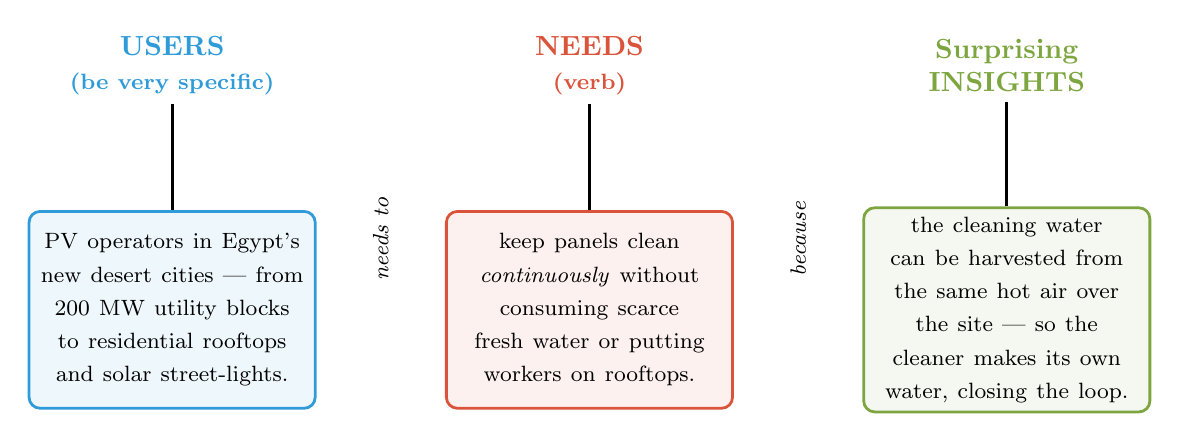
\begin{tikzpicture}[every node/.style={align=center}]
  % column header labels
  \node[text=userblue,font=\bfseries]    (uh) at (-5.3,2.2) {USERS\\\footnotesize(be very specific)};
  \node[text=needred,font=\bfseries]     (nh) at ( 0.0,2.2) {NEEDS\\\footnotesize(verb)};
  \node[text=insightgreen,font=\bfseries](ih) at ( 5.3,2.2) {Surprising\\INSIGHTS};
  % connector vertical labels
  \node[font=\footnotesize\itshape,rotate=90] at (-2.65,0.0) {needs to};
  \node[font=\footnotesize\itshape,rotate=90] at ( 2.65,0.0) {because};
  % filled boxes
  \node[draw=userblue,line width=1pt,rounded corners,fill=userblue!8,
        text width=3.4cm,minimum height=2.5cm] (ub) at (-5.3,-0.9)
        {\footnotesize PV operators in Egypt's new desert cities --- from 200~MW
         utility blocks to residential rooftops and solar street-lights.};
  \node[draw=needred,line width=1pt,rounded corners,fill=needred!8,
        text width=3.4cm,minimum height=2.5cm] (nb) at (0.0,-0.9)
        {\footnotesize keep panels clean \emph{continuously} without consuming scarce
         fresh water or putting workers on rooftops.};
  \node[draw=insightgreen,line width=1pt,rounded corners,fill=insightgreen!8,
        text width=3.4cm,minimum height=2.5cm] (ib) at (5.3,-0.9)
        {\footnotesize the cleaning water can be harvested from the same hot air over
         the site --- so the cleaner makes its own water, closing the loop.};
  % connectors
  \draw[line width=1pt] (uh)--(ub);
  \draw[line width=1pt] (nh)--(nb);
  \draw[line width=1pt] (ih)--(ib);
\end{tikzpicture}
\end{center}

\noindent\colorbox{panelgrey}{\parbox{\dimexpr\linewidth-2\fboxsep}{\small
\textbf{Assembled statement.} \emph{PV operators in Egypt's new desert cities need to
clean their panels continuously --- without consuming scarce fresh water or risking
rooftop labour --- because soiling silently erodes a large share of annual yield while
trucked cleaning water is costly, yet the night air over the very same site can supply
that water for free.}}}

% =====================================================================
%  4. IMPACT STATEMENT
% =====================================================================
\framehead{4.\ \ Impact Statement}{What impact? For whom? How? How measured?}

\noindent\fcolorbox{slideblue}{slideblue!6}{\parbox{\dimexpr\linewidth-2\fboxsep}{%
\small\textbf{If implemented, our project can help} PV operators in Egypt's arid new
cities \textbf{achieve} higher energy yield with near-zero external water use for
cleaning, \textbf{by} deploying an autonomous robot that harvests its own distilled
water from the air (thermoelectric AWH) and cleans panels on schedule, \textbf{leading
to} recovered soiling losses, thousands of cubic metres of trucked water avoided per
year, and zero rooftop labour.}}

\vspace{6pt}
\noindent\begin{tabular}{@{}>{\raggedright}p{3.6cm} >{\raggedright}p{8.0cm} >{\raggedright\arraybackslash}p{4.4cm}@{}}
\toprule
\textbf{Impact indicator} & \textbf{Target for this project} & \textbf{Basis} \\
\midrule
Energy saved / recovered & Recover the bulk of soiling loss; keep panels near-clean year-round & cleaning cadence 18$\times$/yr in the water model \\
Water saved (external) & $\approx$1.8~L/m\textsuperscript{2}/event avoided $\rightarrow$ $\approx$\textbf{37{,}674~m\textsuperscript{3}/yr} for a 200~MW block; prototype self-supplies $\sim$\textbf{200~L/day} & \texttt{project\_inputs.yaml}, \texttt{calculation\_summary} \\
Cost reduced & Avoided water-trucking + cleaning labour; self-generated water LCOW $\approx$\,\textbf{14~USD/m\textsuperscript{3}} (VCR) & \texttt{output/lcow\_table} \\
Safety improved & Workers removed from hot rooftops --- 0 rooftop man-hours & design intent \\
Waste reduced & No detergents; distilled water leaves no residue/streaking & distilled condensate \\
Environmental / health & Less freshwater stress + more clean solar kWh $\rightarrow$ less fossil backup & sustainability framing \\
Number of users served & Scalable across thousands of rooftops + street-lights in NAC / New Alamein / New Mansoura / New Ismailia & 3-scale deployment plan \\
Process efficiency & Continuous autonomous cleaning vs.\ periodic manual crews & autonomy \\
\bottomrule
\end{tabular}

% =====================================================================
%  CLOSING -- riskiest assumption + to-verify
% =====================================================================
\vspace{8pt}
\noindent\fcolorbox{needred}{needred!6}{\parbox{\dimexpr\linewidth-2\fboxsep}{%
\footnotesize\textbf{Riskiest assumption to validate next.} That night-time TEC water
yield, at the site's low-RH hours, actually meets the cleaning-water duty. Cheapest
test: the prototype 24\,h condensate run already planned (milestones M5--M6), logging
litres harvested vs.\ RH and temperature.}}

\vspace{4pt}
\noindent\colorbox{panelgrey}{\parbox{\dimexpr\linewidth-2\fboxsep}{\footnotesize
\textbf{Before you present --- numbers to confirm / insert your cited figure:}
(1)~the soiling energy-loss \% for your site (replace ``a large share'' with your cited
\%/day or \%/yr); (2)~demand evidence from $\geq$3 O\&M / owner interviews;
(3)~the per-scale cost \& payback model (commercial vs.\ residential vs.\ street-lamp).
Quantitative values above are pulled from this project's own files; treat ranges marked
``$\sim$'' as estimates to refine.}}

\end{document}
